
\documentclass[10pt,a4paper]{article}

% Om het totaal aantal pagina's te tellen
\usepackage{lastpage}
\usepackage{graphicx}

% Om de marges aan te passen
\usepackage[left=2cm,right=2cm,top=2cm,bottom=2cm]{geometry}

% Voor headers en footers
\usepackage{fancyhdr}
\pagestyle{fancy}

\lhead{Giuseppe Callari and Xavier Go\'as Aguililla}
\rhead{\thepage /\pageref{LastPage}}

\lfoot{Assignment}
\cfoot{Computer Networks}
\rfoot{Network Simulation}

\renewcommand{\headrulewidth}{0.4pt}
\renewcommand{\footrulewidth}{0.4pt}

\begin{document}
\begin{titlepage}
\thispagestyle{empty}
\newcommand{\HRule}{\rule{\linewidth}{0.5mm}}
\center
\textsc{\LARGE KU Leuven}\\[1.5cm]
\textsc{\Large Assignment:}\\[0.5cm]
\textsc{\large Network Simulation}\\[0.5cm]

\HRule \\[0.4cm]
{ \Huge \bfseries Report}\\[0.4cm]
\HRule \\[1.5cm]

\begin{minipage}{0.4\textwidth}
\begin{flushleft} \large
\emph{Authors:}\\
Giuseppe \textsc{Callari}\\
Xavier \textsc{Go\'as Aguililla}
\end{flushleft}
\end{minipage}
~
\begin{minipage}{0.4\textwidth}
\begin{flushright} \large
\emph{Professor:} \\
prof. dr. D. \textsc{Hughes}
\end{flushright}
\end{minipage}\\[4cm]

{\large May 2nd, 2014}\\[3cm]
\vfill

\end{titlepage}


\section{Exercise 1}
\subsection{Question 1}

\begin{figure}[p]
    \centering
    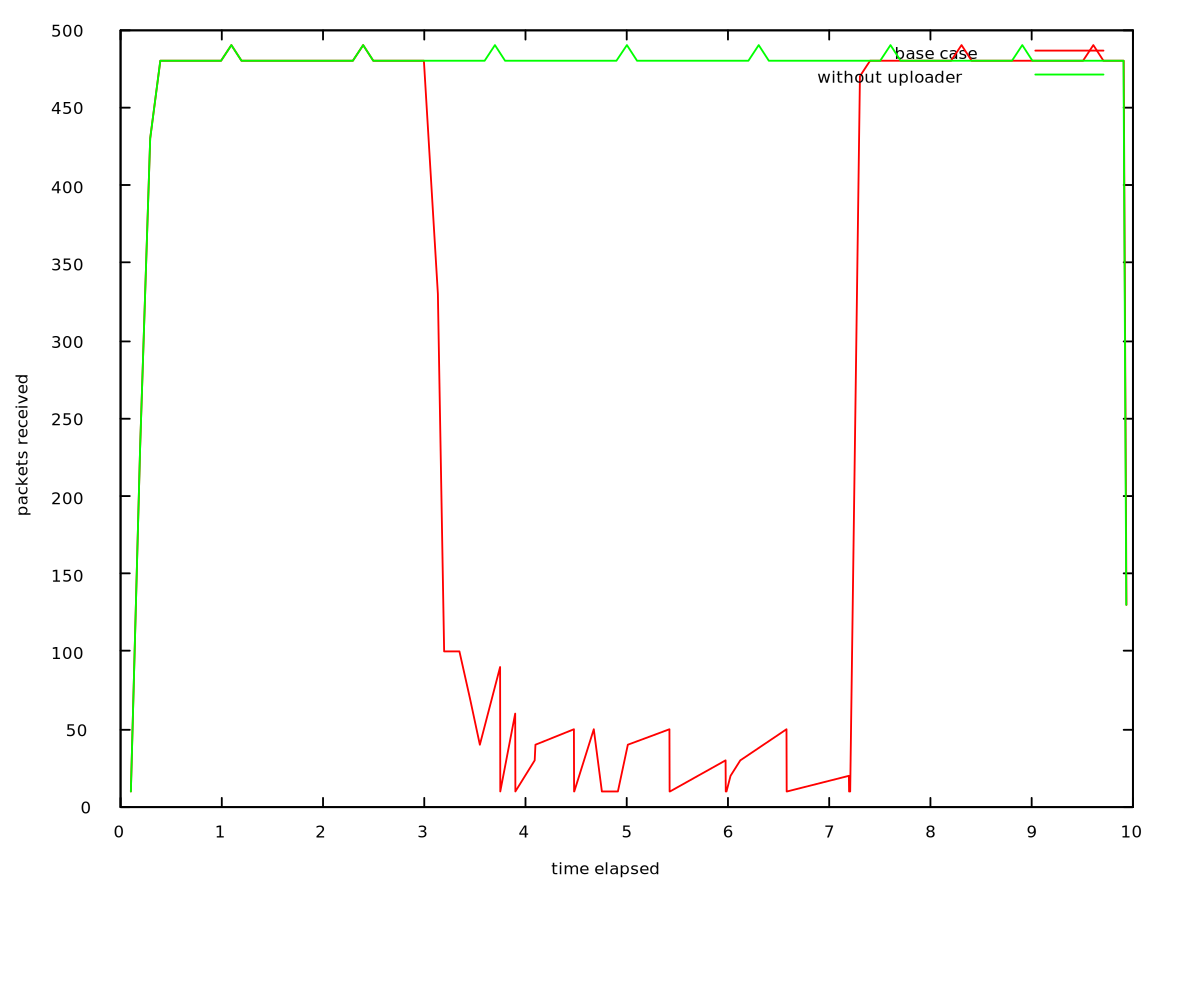
\includegraphics[width=\textwidth]{../part1/q1/plots/1.pdf}
    \caption{Surprise muthafucka}
    \label{fig:awesome_image}
\end{figure}

\subsection{Question 2}
\subsection{Question 3}
\subsection{Question 4}
\begin{figure}[p]
    \centering
    \includegraphics[width=\textwidth]{../part1/q4/plots/4.pdf}
    \caption{Surprise muthafucka, the return}
    \label{fig:awesome_image_2}
\end{figure}
\subsection{Question 5}
\subsection{Question 6}

\section{Exercise 2}
\subsection{Question 1}
\subsection{Question 2}
\subsection{Question 3}
\subsection{Question 4}

\end{document}